\documentclass{AeroStructure-ERJohnson}
\input crosslink.tex

%\usepackage{showframe}
\def\ShowFrameLinethickness{0.125pt}

\def\harp#1{\smash{\mathord{\buildrel{\lower3pt\hbox{$\scriptscriptstyle\rightharpoonup$}}\over{#1}}}}


\myexternaldocument{App_4P}
\myexternaldocument{Ch01_4P}
%\myexternaldocument{Ch02_4P}
\myexternaldocument{Ch03_4P}
\myexternaldocument{Ch04_4P}
\myexternaldocument{Ch05_4P}
\myexternaldocument{Ch06_4P}
\myexternaldocument{Ch07_4P}
\myexternaldocument{Ch08_4P}
\myexternaldocument{Ch09_4P}
\myexternaldocument{Ch10_4P}
\myexternaldocument{Ch11_4P}
\myexternaldocument{Ch12_4P}
\myexternaldocument{Ch13_4P}
\myexternaldocument{Ch14_4P}
\myexternaldocument{Ch15_4P}
\myexternaldocument{Ch16_4P}
\myexternaldocument{Ch17_4P}
\myexternaldocument{Ch18_4P}

\begin{document}


\mainmatter
\setcounter{page}{7}

\setcounter{chapter}{1}

\chapter{Aircraft loads}\label{ch2}

Consider an airplane moving through calm air. Particles of air affected by the airplane are accelerated and the reaction of the accelerated particles is felt over the surfaces of the airplane as a distribution of pressures. The pressure distribution acting on the surfaces of the airplane can be resolved into the total lift and drag forces. In addition to the aerodynamic forces of lift and drag, there are so-called inertia loads resulting from the acceleration of the airplane. Other loading conditions such as landing loads, ground-handling loads, horizontal and vertical tail loads, and monocoque body loads are discussed in detail by Lomax (1996).

Load analysis is important in aircraft design, and a design cannot proceed without information on loads. The aircraft loads analysis presented in this chapter is used in preliminary design, which is defined in the next section. In this chapter we define load factors, discuss the aerodynamic data required for structural analysis, develop the basic maneuver V-n diagram, and discuss gust load factors used in design.

\section{Aircraft design process}\label{sec2.1}

Phases of the aircraft design may be divided into a concept formulation, a concept design, a preliminary design, and a detail design. Concept formulation is where the basic requirements for new aircraft are developed. Requirements are developed by a combination of market and customer surveys, and statistical analyses. Concept design begins with the basic requirements and sizes the aircraft. Only the most simple analysis methods and historical data are used. In preliminary design the sized conceptual baseline aircraft is further developed. Increased level of analysis is used to define the aerodynamics, performance, weight, propulsion, acoustic and cost parameters of the design. Detailed design is where the various parts of the aircraft are designed for fabrication. Part and assembly drawings are developed for manufacturing.

\section{Inertia loads}\label{sec2.2}

The maximum load on any part of the airplane structure occurs when it accelerates. In preliminary design, inertia force calculations are usually based on rigid body dynamics of the airplane. Once these loads are determined they are imposed on the airplane, and the structural design proceeds by assuming the airplane is flexible (i.e., a deformable body). Determining inertia loads for a deformable body is more complex, and may be warranted later in the structural design process.

\subsection{Coordinate systems and Newton's laws of motion}\label{sec2.2.1}

The right-handed Cartesian coordinate system O\textit{XYZ} is fixed to the Earth, origin at point O, and it is assumed that this is an inertial system. That is, Newton's laws of motion are valid in the Earth axis system. The unit base vectors in the O\textit{XYZ} system are denoted by $(\hat{I}, \hat{J}, \hat{K})$. The right-handed Cartesian coordinate system \textit{Gxyz} is fixed in the body of the aircraft, with its origin at the center of gravity, which is labeled \textit{G. }The unit base vectors in the \textit{Gxyz} system are denoted by $(\hat{i}, \hat{j}, \hat{k})$. Consider planar motion of the aircraft -- that is, symmetrical maneuvers of the aircraft, and where the aircraft is symmetrical about its vertical fore and aft plane. Body axis \textit{Gx} is directed forward, axis \textit{Gy} is directed toward the starboard wing, and body axis \textit{Gz} is in the normal direction. For symmetrical maneuvers there is no roll or yaw of the airplane, so symmetrical maneuvers imply $\hat{j}=\hat{J}$ for all time \textit{t}. Let $\harp{R}_{G}$ denote the position vector of the center of gravity \textit{G} with respect to fixed point O. The flight path is a plane curve in the \textit{X-Z} plane with the arc-length along the curve denoted by \textit{s}. The unit tangent vector to the flight path at \textit{s} is denoted by $\hat{t}$, the unit normal vector at \textit{s} by $\hat{n}$, and the angle between the flight path and the unit tangent vector, or the x-axis, by $\theta$. Note that $\hat{t}=\hat{i}$. Angle $\theta$ represents the clockwise rotation of the aircraft in pitch. See figure~\ref{fig2.1}.

{\def\thefigure{2.1}
\processfigure{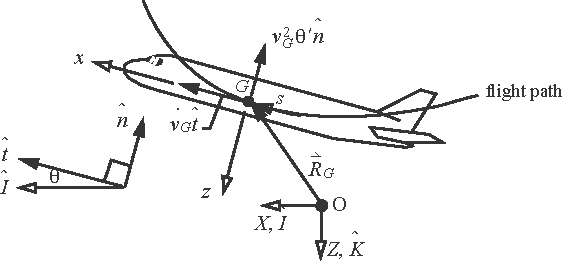
\includegraphics{Figure_2-1.pdf}
}{\caption{Acceleration of the center of gravity tangent and normal to the flight path.\label{fig2.1}}}}



The unit tangent vector and its derivative along the path are
\begin{align}\label{eq2.1}
\hat{t}=\frac{d \harp{R}_{G}}{d s}\mbox{, and }\frac{d \hat{t}}{d s}=\frac{d \theta}{d s} \hat{n}.
\end{align}
Let $\theta^{\prime}=d \theta/d s$. The change in slope of the flight path with respect to arc-length $\theta^{\prime}$ defines the curvature of the path, and the radius of curvature is $R=1/\theta^{\prime}$. The velocity of the center of gravity \textit{G} along the flight path is
\begin{align}\label{eq2.2}
\harp{v_{G}}=\frac{d \harp{R}_{G}}{d t}=\frac{d \harp{R}_{G}}{d s} \frac{d s}{d t}=\hat{t} v_{G},
\end{align}
where the speed of the center of gravity of the aircraft along the flight path is $v_{G}=d s/d t$. The acceleration of the center of gravity is
\begin{align}\label{eq2.3}
\harp{a_{G}}=\frac{d \harp{v_{G}}}{d t}=\frac{d}{d t}(v_{G} \hat{t})=\dot{v}_{G} \hat{t}+v_{G} \frac{d \hat{t}}{d s} \frac{d s}{d t}=\dot{v}_{G} \hat{t}+v_{G}^{2} \theta^{\prime} \hat{n}.
\end{align}
where $\dot{v}_{G}=d v_{G}/d t$ is the acceleration component tangent to the path. The acceleration component normal to the path $v_{G}^{2} \theta^{\prime}=v_{G}^{2}/R$, or centripetal acceleration, is directed toward the concave side of the path.

A free body diagram of the aircraft at time \textit{t} and its time rate of change of momenta are shown in figure \ref{fig2.2}.

{\def\thefigure{2.2}
\processfigure{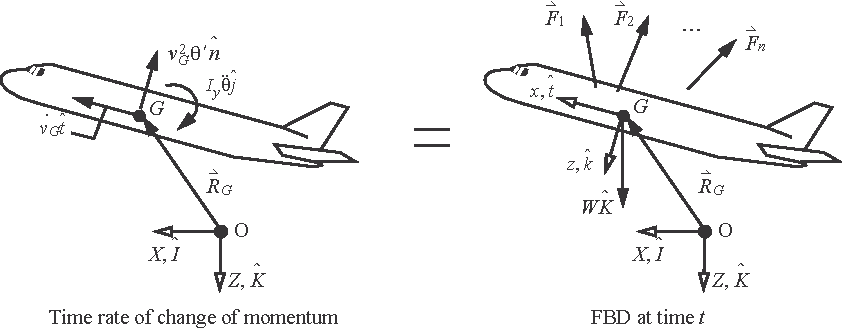
\includegraphics{Figure_2-2.pdf}
}{\caption{Free body and rate of momenta diagrams for symmetrical motion of an aircraft at time $t$.\label{fig2.2}}}}


Derivatives with respect to time of the pitch angle are written as
\begin{align}\label{eq2.4}
\frac{d \theta}{d t}=\dot{\theta}\mbox{, and }\frac{d^{2} \theta}{d t^{2}}=\ddot{\theta}.
\end{align}
The mass of the aircraft is denoted by \textit{m}, the moment of inertia about the center of gravity by $I_{y}$, the local acceleration due to gravity by $g$, and the weight of the aircraft by \textit{W} where $W=m g$. Equations for Newton's second law at time \textit{t} are
\begin{align}\label{eq2.5}
\harp{F}=m\big(\dot{v}_{G} \hat{t}+v_{G}^{2} \theta^{\prime} \hat{n}\big) \quad \harp{M}_{G}=I_{y} \ddot{\theta} \hat{j} \quad \harp{M}_{\mathrm{O}}=\harp{R}_{G} \times m\big(\dot{v_{G}} \hat{t}+v_{G}^{2} \theta^{\prime} \hat{n}\big)+I_{y} \ddot{\theta} \hat{j},
\end{align}
where the resultant force is denoted by $\harp{F}$, the moment about the center of gravity by $\harp{M}_{G}$, and the moment about the fixed point by $\harp{M}_{\mathrm{O}}$. These force and moment vectors are determined from
\begin{align}\label{eq2.6}
\harp{F}=\sum_{m=1}^n \harp{F}_{m} \quad \harp{M}_{G}=\sum_{m=1}^n \harp{r}_{m/G} \times \harp{F}_{m} \quad \harp{M}_{\mathrm{O}}=\harp{M}_{G}+\harp{R}_{G} \times \harp{F},
\end{align}
where $\harp{r}_{m/G}$ is the position vector of the point of application of force $\harp{F}_{m}$ with respect to the center of gravity.

\subsection{Principle of D'Alembert}\label{sec2.2.2}

D'Alembert in 1743 proposed a principle that would reduce a problem in dynamics to an equivalent one in statics by introducing so-called \textit{inertial forces}. The inertial force acting at the airplane's center of gravity is defined as $-m \harp{a}_{G}$, and the inertial moment about the center of gravity is defined as $-I_{y} \ddot{\theta} \hat{j}$. These inertial forces are drawn on the free body diagram of the airplane in addition to all the applied forces. \textit{D'Alembert's principle states that the applied forces together with the inertial forces form a system in equilibrium. }Thus we write Newton's second law~as
\begin{align}\label{eq2.7}
\harp{F}+\big(-m \dot{v}_{G} \hat{t}-m v_{G}^{2} \theta^{\prime} \hat{n}\big)=0 \quad \harp{M}_{G}+\big(-I_{y} \ddot{\theta} \hat{j}\big)=0.
\end{align}
The free body diagram is modified accordingly as shown in figure \ref{fig2.3}. In the free body diagram the inertial forces and moment are indicated by dashed lines. From the free body diagram we proceed as in statics to write the conditions of (dynamic) equilibrium.


{\def\thefigure{2.3}
\processfigure{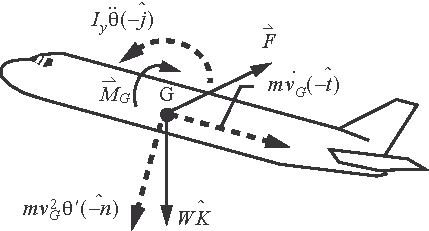
\includegraphics{Figure_2-3.pdf}
}{\caption{Aircraft free body diagram at time $t$ including the inertial forces and the inertial moment.\label{fig2.3}}}}





The curvature of the flight path $\theta^{\prime}$ can change sign. As shown in figure \ref{fig2.4}, the curvature is positive for a pull-up maneuver from a dive, and the curvature is negative for a push-down maneuver from a climb. Consequently, the inertia force normal to the flight path is directed toward the convex side of the path.

{\def\thefigure{2.4}
\processfigure[H]{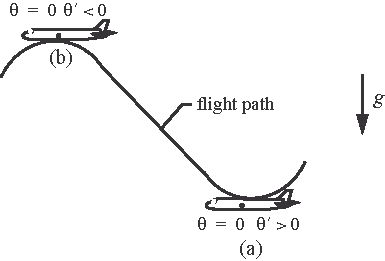
\includegraphics{Figure_2-4.pdf}
}{\caption{Sign of the curvature for (a) pull-up from a dive, and (b) push-down from a climb.\label{fig2.4}}}}


\subsection{Relative velocity and acceleration}\label{sec2.2.3}

Often it is necessary to determine the inertial forces at locations within the airplane not coincident with the center of gravity. For these computations we need the relative velocity and acceleration formulas from rigid body dynamics. Consider two points \textit{A} and \textit{G} fixed in the body. The position of point \textit{A} relative to \textit{G} is taken as $x_{A/G} \hat{i}$, as shown in figure \ref{fig2.5}.

{\def\thefigure{2.5}
\processfigure[H]{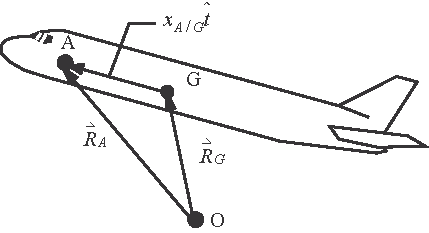
\includegraphics{Figure_2-5.pdf}
}{\caption{Relative position of two points fixed in a rigid body.\label{fig2.5}}}}


The position vectors of points \textit{A} and \textit{G} are related by
\begin{align}\label{eq2.8}
\harp{R}_{A}=\harp{R}_{G}+x_{A/G} \hat{i}.
\end{align}
The velocity vectors of points \textit{A} and \textit{G} are then
\begin{align}\label{eq2.9}
\harp{v}_{A}=\harp{v}_{G}+\frac{d}{d t}(x_{A/G} \hat{t}).
\end{align}
Since vector $x_{A/G} \hat{i}$ is embedded in the rigid body for all time, its rate of change is determined from its cross product with the vector of the time rate of change of pitch rotation. That is,
\begin{align}\label{eq2.10}
\frac{d}{d t}(x_{A/G} \hat{t})=\dot{\theta} \hat{j} \times x_{A/G} \hat{t}=x_{A/G} \dot{\theta} \hat{n}.
\end{align}
Hence,
\begin{align}\label{eq2.11}
\harp{\nu}_{A}=\harp{\nu}_{G}+ x_{A/G} \dot{\theta} \hat{n}.
\end{align}
The time rate of change of this velocity expression (2.11) relates the acceleration of \textit{A} relative to \textit{G} by
\begin{align}\label{eq2.12}
\harp{a}_{A}=\harp{a}_{G}+\frac{d}{d t}[x_{A/G} \dot{\theta} \hat{n}]=\harp{a}_{A}+x_{A/G} \ddot{\theta} \hat{n}+\dot{\theta} \frac{d}{d t}[x_{A/G} \hat{n}]=\harp{a}_{G}+x_{A/G} \ddot{\theta} \hat{n}+\dot{\theta}[\dot{\theta} \hat{j} \times x_{A/G} \hat{n}].
\end{align}
Perform the vector cross product in eq. (2.12) to find
\begin{align}\label{eq2.13}
\harp{a}_{A}=\harp{a}_{G}+x_{A/G} \ddot{\theta} \hat{n}-\dot{\theta}^{2} x_{A/G} \hat{t}.
\end{align}

\subsection{Uniform linear and angular accelerations}\label{sec2.2.4}

In some inertial load problems it is reasonable to assume that the acceleration of a particle and/or the angular acceleration of a rigid body are constant over a time interval. Let \textit{s} denote the distance of a particle along a straight line, \textit{v} its speed along the line, and \textit{a }its constant acceleration. Then, we have the following formulas
\begin{align}\label{eq2.14}
v=a t+v_{0} \quad s=\frac{1}{2} a t^{2}+v_{0} t+s_{0} \quad 2 a\left(s-s_{0}\right)=v^{2}-v_{0}^{2},
\end{align}
where $s=s_{0}$ and $\nu=v_{0}$ at time $t=0$. Similarly if the angular acceleration $\ddot{\theta}$ is constant over some time interval, then
\begin{align}\label{eq2.15}
\dot{\theta}=\ddot{\theta} t+\dot{\theta}_{0} \quad \theta=\frac{1}{2} \ddot{\theta} t^{2}+\dot{\theta}_{0} t+\theta_{0} \quad 2 \ddot{\theta}\left(\theta-\theta_{0}\right)=\dot{\theta}^{2}-\dot{\theta}_{0}^{2},
\end{align}
where $\dot{\theta}=\dot{\theta}_{0}$ and $\theta=\theta_{0}$ at time $t=0$.

\section{Load factors}\label{sec2.3}

It is convenient to combine the inertial forces and gravity forces in the analysis of aircraft structural components. Consider an airplane in general plane motion as depicted in figure \ref{fig2.6}.

{\def\thefigure{2.6}
\processfigure[H]{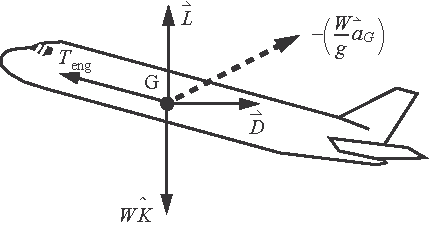
\includegraphics{Figure_2-6.pdf}
}{\caption{Inertial force, weight, and other forces acting on an airplane in general plane motion.\label{fig2.6}}}}



The actions shown in figure \ref{fig2.6} represent: $\harp{L}$ = lift force (wing and tail), $\harp{D}$ = drag force, $\harp{T}_{\text {eng }}$ = thrust force, $-\frac{W}{g} \harp{a}_{G}$ = inertia force, and $\harp{a}_{G}$ = acceleration of the center of gravity given by eq. (\ref{eq2.3}). We are not considering the moment of momentum equation for now. However, $\ddot{\theta} \neq 0$ in general. For the configuration shown in figure \ref{fig2.6} dynamic equilibrium is
\begin{align}\label{eq2.16}
\harp{L}+\harp{D}+\harp{T}_{\text {eng }}+W \hat{K}-\frac{W}{g} \harp{a}_{G}=0.
\end{align}
Let the total applied force on the airplane excluding weight be noted by $\sum {\harp{F}}$. The total applied force, in general, may include other effects than those shown in the sketch above (e.g., wheel reactions on landing.) Then dynamic equilibrium is written as
\begin{gather}\label{eq2.17}
\sum \harp{F}-\underbrace{\left[-W \hat{K}+\frac{W}{g} \harp{a}_{G}\right]}=0. \nonumber\\
\mbox{combined weight and inertia force}
\end{gather}

%{\def\thefigure{2.7}
\begin{wrapfigure}[6]{r}{64pt}
\vspace*{-18pt}
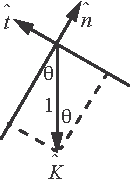
\includegraphics{Figure_2-7.pdf}
\caption{\label{fig2.7}}
\end{wrapfigure}
%}


\noindent As shown in figure \ref{fig2.7}, the projection of the gravity unit vector on the tangent and normal directions is $\hat{K}=\sin \theta(-\hat{t})+\cos \theta(-\hat{n})$. Similarly, we define the projections of the resultant forces in the tangent and normal directions as
\begin{align}\label{eq2.18}
\sum \harp{F} \cdot \hat{t}=\left(\sum F\right)_{x} \quad \sum \harp{F} \cdot \hat{n}=\left(\sum F\right)_{n}.
\end{align}
Dynamic equilibrium (\ref{eq2.17}) separated into tangent and normal directions is
\begin{align}\label{eq2.19}
\left[\left(\sum F\right)_{x}-W\left(\sin \theta+\frac{\dot{v}_{G}}{g}\right)\right] \hat{t}+\left[\left(\sum F\right)_{n}-W\left(\cos \theta+\frac{v_{G}^{2} \theta^{\prime}}{g}\right)\right] \hat{n}=0.
\end{align}
Rewrite dynamic equilibrium (\ref{eq2.19}) in the form
\begin{align}\label{eq2.20}
\left[\left(\sum F\right)_{x}-n_{x} W\right] \hat{t}+\left[\left(\sum F\right)_{n}-n_{z} W\right] \hat{n}=0,
\end{align}
where the load factors in the tangent and normal directions are defined by
\begin{align}\label{eq2.21}
\boxed{n_{x} \equiv\left(\sin \theta+\frac{\dot{v}_{G}}{g}\right) \qquad n_{z}=\left(\cos \theta+\frac{v_{G}^{2} \theta^{\prime}}{g}\right).}
\end{align}
Also, eq. (2.20) shows that the load factors can be determined from
\begin{align}\label{eq2.22}
\boxed{n_{x}=\left(\sum F\right)_{x}/W \qquad n_{z}=\left(\sum F\right)_{n}/W.}
\end{align}
Note that the load factor is a dimensionless number, and it can be negative, zero, or positive. The free body diagram for dynamic equilibrium of the airplane employing load factors is shown in figure \ref{fig2.8}.

{\def\thefigure{2.8}
\processfigure[H]{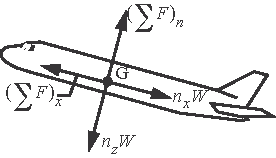
\includegraphics{Figure_2-8.pdf}
}{\caption{Inertial forces and gravity forces represented by load factors for dynamic equilibrium of the airplane.\label{fig2.8}}}}


\section{The V-n diagram}\label{sec2.4}

First, some definitions:
\begin{unlist}
\item[Limit load] -- the maximum load that an aircraft may be expected to encounter at any time in service

\item[Limit load factor] -- \textit{n} associated with limit load $n W=L L$

\item[Ultimate load] -- force necessary to rupture

\item[Ultimate load factor] -- \textit{n} associated with ultimate load $n W=U L$

\item[Factor of safety] -- ultimate load/limit load > 1; usually 1.5
\end{unlist}

\subsection{Airplane design requirements}\label{sec2.4.1}
\vspace*{12pt}
\begin{framed}
\begin{enumerate}
\vspace*{-12pt}
\item[1.] All parts of the airplane are designed so they are not stressed beyond the yield point at the limit load factor.

\item[2.] The airplane structure must carry the ultimate loads for at least 3 seconds without collapsing, even though the members may acquire permanent deformation.
\end{enumerate}
\vspace*{-1\topsep}%
\end{framed}

\subsection{Regulations}\label{sec2.4.2}

Limit load factors are specified by regulations, which depend on the type of aircraft (e.g., transport, aerobatic, etc.). Criteria for civil aerospace vehicles in the United States.

\begin{unlist}
  \item[] Code of Federal Regulations
  \item[] \qquad Title 14, Aeronautics and Space
  \item[] \qquad Parts 1--59
  \item[] Federal Aviation Administration (Department of Transportation is the regulatory agency.)
  \item[] Military requirements in the United States. issued in \textbf{MIL--Specs} covering specific topics of structural design\break \hspace*{-15pt}of US Air Force, Navy, and Marine aircraft.
\end{unlist}

\subsection{Specified data}\label{sec2.4.3}

Specified maximum positive load factor; $n_{\max }>1$.\\
Specified maximum negative load factor; $n_{\min }<0$.\\
Specified design airspeeds:
\begin{gather*}
V_{C}=\text{maximum level flight cruise speed }\\
V_{D}=\text { maximum dive speed } \sim 1.2 \text { to } 1.5 V_{C}
\end{gather*}

\subsection{Basic maneuver V-n diagram}\label{sec2.4.4}

This is predicated on pilot-controlled, symmetrical maneuvers in flight through calm air (i.e., no gust). Assumptions made for analytical purposes are that the pitching acceleration is assumed zero or negligible, the airspeed is constant during the maneuver, and there is no rolling or yawing of the aircraft, although rolling or yawing maneuvers may be considered in design as well. For no pitching acceleration the pitch rate $\dot{\theta}$ is constant with respect to time. Use the chain rule to write the pitch rate as
\begin{align}\label{eq2.23}
\dot{\theta}=\frac{d \theta}{d t}=\frac{d \theta}{d s} \frac{d s}{d t}=\theta^{\prime} v_{G}.
\end{align}
Hence, in a steady state maneuver $\theta^{\prime} v_{G}$ is constant with respect to time. The load factors (\ref{eq2.21}) for a steady state maneuver are
\begin{align}\label{eq2.24}
n_{x}=\sin \theta \quad n_{z}=\left(\cos \theta+\frac{v_{G}^{2} \theta^{\prime}}{g}\right).
\end{align}
A pull-up from a dive, and a push-down from a climb are examples of steady state symmetrical maneuvers and are depicted in figure \ref{fig2.4}. Also, a level flight, coordinated turn is considered a symmetrical maneuver even though the airplane does have a lateral acceleration in the turn. (Refer to practice exercise 2.) In general, the steady state symmetrical maneuvers will produce the maximum design wing loads. See figure \ref{fig2.9}.


{\def\thefigure{2.9}
\processfigure{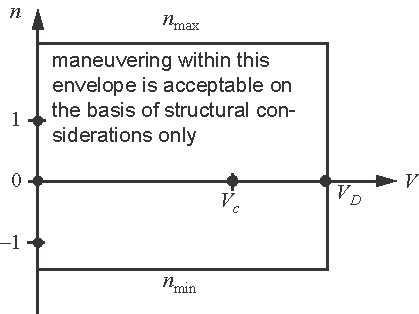
\includegraphics{Figure_2-9.pdf}
}{\caption{Maneuver V-n diagram based on structural considerations only.\label{fig2.9}}}}



\subsection{Aerodynamic data}\label{sec2.4.5}

When a two-dimensional airfoil is subject to a relative wind there is a net pressure distribution over the airfoil that depends on the angle of attack, which is denoted by $\alpha$. The angle of attack is the angle between the relative wind and the chord of the airfoil.The chord is the width of the airfoil and its length is denoted by \textit{c}. The resultant action of the pressure distribution is a force \textit{R} and no moment at the center of pressure, which is labeled C.P. in figure \ref{fig2.10}(a). The center of pressure location varies with the angle of attack. The resultant action of the pressure distribution is a force and a moment at any other location. The standard reference point for aerodynamic data is the aerodynamic center, which is labeled A.C. in figure \ref{fig2.10}(b). The aerodynamic center is the point where the pitching moment is independent of the angle of attack. For most subsonic wing sections the A.C. is around 25 percent of the chord.The net force of the pressure distribution is resolved at the aerodynamic center into a lift force perpendicular to the relative wind and a drag force parallel to the relative wind and the pitching moment.


{\def\thefigure{2.10}
\processfigure{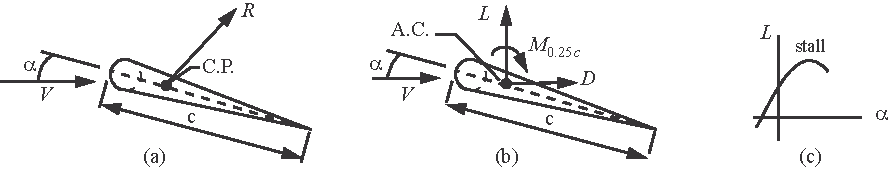
\includegraphics{Figure_2-10.pdf}
}{\caption{Characteristics of a two-dimensional airfoil: (a) center of pressure, (b) aerodynamic center, (c) stall.\label{fig2.10}}}}



The lift increases as the angle of attack increases. At some point, however, the flow can no longer stay attached to the upper surface and detaches. This results in a decrease in lift, which is called \textbf{aerodynamic stall} as shown in figure \ref{fig2.10}(c). The sharpness of the decrease in lift is dependent on the type of airfoil\vadjust{\vfill\pagebreak}.

Airplanes are three-dimensional vehicles with three-dimensional aerodynamic surfaces, so the aerodynamic loads are spread over these surfaces. This distribution in the spanwise direction of the wing results in a force and moment at the root of the wing. The spanwise distribution of the airload is a function of the wing planform shape, the airfoil sections, and the geometric twist. The basic aerodynamic reference for three-dimensional wings is the \textbf{mean aerodynamic chord} (MAC). The thickness, chord length, and angle of attack of the MAC airfoil section is used as a reference for all aerodynamic data. For a rectangular wing planform, the MAC is equal to the wing chord, and for a trapezoidal planform of the semiwing the MAC is equal to the chord at the centroid of the trapezoid.

\vspace*{-10pt}

\paragraph{Methods of data acquisition.}

Basic methods to calculate aerodynamic data for aircraft design and analysis are preliminary design estimates, wind tunnel testing, numerical fluid analysis, and aircraft flight test. The wind tunnel test is the major source for aerodynamic data in the preliminary design phase, and it involves construction of a scale model of the aircraft. The model is instrumented with pressure and force transducers. Data required for the structural analysis are the lift, drag, and pitching moment curves for the complete airplane with the horizontal tail removed through the range of angles of attack from the negative stalling angle to the positive angle. Data for the combination of the wing and fuselage, or the wing, fuselage, and nacelles, are more difficult to calculate accurately from the published data, because of the uncertain effects of the aerodynamic interference of the various components.

The lift force \textit{L} is normal to the relative velocity (flight path), the drag force \textit{D} is parallel to the relative velocity, and the pitching moment $M_{0.25}$ is nose-up positive at the mean aerodynamic chord as shown in figure \ref{fig2.11}(a). The angle $\theta$ is measured from the flight path to the \textit{x}-axis and is equal to the difference between to the angle of attack $\alpha$ and the angle of wing incidence \textit{i}.

{\def\thefigure{2.11}
\processfigure{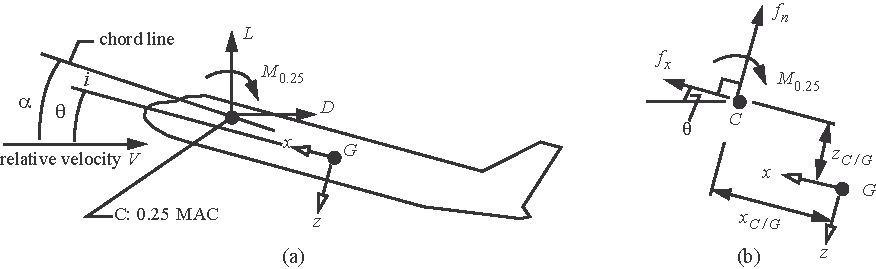
\includegraphics{Figure_2-11.pdf}
}{\caption{(a) Lift force, drag force, and pitching moment at the MAC. (b) Lift and drag resolved along the body x- and z-axes at MAC.\label{fig2.11}}}}

\vspace*{10pt}

\pagebreak

The lift force, drag force, and pitching moment for the tail-off are expressed in terms of the dynamic pressure \textit{q}, wing reference area \textit{S}, and dimensionless aerodynamic coefficients $C_{L}$, $C_{D}$, and $C_{M 0.25}$. The dynamic pressure~is
\begin{align}\label{eq2.25}
q=\frac{1}{2} \rho V^{2},
\end{align}
where the air density at altitude is denoted by $\rho$. The aerodynamic actions are expressed as
\begin{align}\label{eq2.26}
L=C_{L} q S \qquad D=C_{D} q S \qquad M_{0.25}=C_{M 0.25} q S \bar{c},
\end{align}
where the mean aerodynamic chord is denoted by $\bar{c}$.

The aerodynamic actions \textit{L}, \textit{D}, and $M_{0.25}$ at the mean aerodynamic chord are statically equivalent to the aerodynamic actions $f_{n}$, $f_{x}$, and $M_{y}$ at the center of gravity. The lift and drag forces are resolved into components normal $f_{n}$ and parallel $f_{x}$ to the flight path by
\begin{align}\label{eq2.27}
f_{n}=L \cos \theta+D \sin \theta\mbox{, and }f_{x}=L \sin \theta-D \cos \theta.
\end{align}
The moment at the center of gravity is determined from figure \ref{fig2.11}(b):
\begin{align}\label{eq2.28}
M_{y}=M_{0.25}+x_{C/G} f_{n}-z_{C/G} f_{x}.
\end{align}
The forces acting on the airplane are shown in figure \ref{fig2.12}, in which the tail force $L_{t}$ acts perpendicular to the flight path at the center of pressure of the horizontal tail.


{\def\thefigure{2.12}
\processfigure{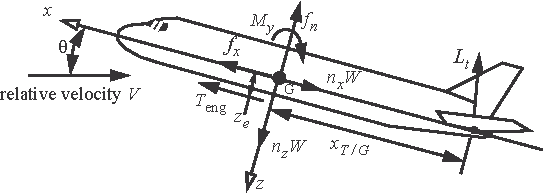
\includegraphics{Figure_2-12.pdf}
}{\caption{Forces acting on the airplane during steady state symmetrical maneuvers. No pitching acceleration.\label{fig2.12}}}}


The dynamic equilibrium equations for no acceleration in pitch are
\begin{align}
f_{x}+T_{\text {eng }}-n_{x} W+L_{t} \sin \theta=0,\label{eq2.29}\\
f_{n}-n_{z} W+L_{t} \cos \theta=0\mbox{, and}\label{eq2.30}\\
M_{y}+z_{e} T_{\text {eng }}-x_{T/G} L_{t} \cos \theta=0.\label{eq2.31}
\end{align}
Substitute the moment at the center of gravity (\ref{eq2.28}) into eq. (\ref{eq2.31}) to get
\begin{align}\label{eq2.32}
M_{0.25}+x_{C/G} f_{n}-z_{C/G} f_{x}+z_{e} T_{e n g}-x_{T/G} L_{t} \cos \theta=0.
\end{align}

Introduce aerodynamic coefficients $C_{n}$, $C_{x}$ and $C_{t}$ by the relations
\begin{align}\label{eq2.33}
f_{n}=C_{n} q S, f_{x}=C_{x} q S\mbox{,  and }L_{t}=C_{t} q S.
\end{align}
Substituting $f_{n}$ and $f_{x}$ from the definitions (\ref{eq2.33}) into eq. (\ref{eq2.27}) determines the coefficients $C_{n}$ and $C_{x}$ as
\begin{align}\label{eq2.34}
C_{n}=C_{L} \cos \theta+C_{D} \sin \theta\mbox{, and }C_{x}=C_{L} \sin \theta-C_{D} \cos \theta.
\end{align}
The balancing tail force coefficient $C_{t}$ is to be determined from the equations of dynamic equilibrium. From the relations (\ref{eq2.33}) and (\ref{eq2.34}), the equilibrium equations (\ref{eq2.29}) and (\ref{eq2.30}) are written~as
\begin{align}\label{eq2.35}
n_{x} W=\left(C_{x}+C_{t} \sin \theta\right) q S+T_{\text {eng }}\mbox{, and}\\
n_{z} W=\left(C_{n}+C_{t} \cos \theta\right) q S.\label{eq2.36}
\end{align}
Let $n_{z} W=C_{N} q S$, where the airplane normal coefficient is denoted by $C_{N}$. From eq. (\ref{eq2.36}) the normal coefficient~is
\begin{align}\label{eq2.37}
C_{N}=C_{n}+C_{t} \cos \theta.
\end{align}
In terms of the aerodynamic relations introduced, the moment about the center of gravity (\ref{eq2.32}) is
\begin{align}\label{eq2.38}
C_{M 0.25} q S \bar{c}+x_{C/G} C_{n} q S-z_{C/G} C_{x} q S+z_{e} T_{e n g}-x_{T/G} C_{t} q S \cos \theta=0.
\end{align}
Rearrange eq. (\ref{eq2.38}) to
\begin{align}\label{eq2.39}
(C_{M 0.25} \bar{c}+x_{C/G} C_{n}-z_{C/G} C_{x}-x_{T/G} C_{t} \cos \theta) q S+z_{e} T_{\text {eng }}=0.
\end{align}
Consider the case of power-off so that $T_{\text {eng }}=0$, and solve for $C_{t} \cos \theta$ to get
\begin{align}\label{eq2.40}
C_{t} \cos \theta=(\bar{c}/x_{T/G}) C_{M 0.25}+(x_{C/G}/x_{T/G}) C_{n}-(z_{C/G}/x_{T/G}) C_{x}.
\end{align}
If the term on the right side containing longitudinal coefficient $C_{x}$ is assumed small with respect to the other terms and neglected, then the resulting expression for coefficient $C_{t}$ is consistent with the traditional equation for the balancing tail load (Lomax, p. 9). Substitute $C_{t} \cos \theta$ from eq. (\ref{eq2.40}) into eq. (\ref{eq2.37}) to get the expression for the normal coefficient determined from the aerodynamic coefficients with the tail off:
\begin{align}\label{eq2.41}
C_{N}=(\bar{c}/x_{T/G}) C_{M 0.25}+(x_{C/G}/x_{T/G}) C_{n}-(z_{C/G}/x_{T/G}) C_{x}.
\end{align}
The total normal force is denoted by $L_{z}$. From eq. (2.30) $L_{z}=f_{n}+L_{t} \cos \theta=n_{z} W$, and $n_{z} W=C_{N} q S$. Hence,
\begin{align}\label{eq2.42}
L_{z}=n_{z} W=C_{N} q S=\left(\frac{1}{2} \rho V^{2}\right) S C_{N}.
\end{align}
\noindent From wind tunnel data for complete airplane the aerodynamic coefficient of lift along the \textit{z} axis is plotted against the angle of attack as depicted in figure \ref{fig2.13}. Generally, the magnitudes of the maximum and minimum values of the normal aerodynamic coefficient corresponding to stall and inverted stall, respectively, satisfy
\begin{align*}
\left|\left(C_{N}\right)_{\min }\right|<\left|\left(C_{N}\right)_{\max }\right|.
\end{align*}
{\def\thefigure{2.13}
\processfigure{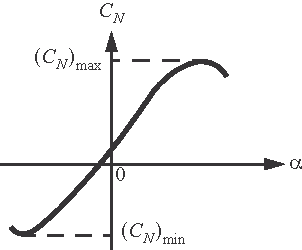
\includegraphics{Figure_2-13.pdf}
}{\caption{Normal force coefficient as a function of the angle of attack.\label{fig2.13}}}}
\noindent Substitute $C_{x}$ from eq. (\ref{eq2.34}) into eq. (\ref{eq2.35}) to find the longitudinal load factor as
\begin{align}\label{eq2.43}
n_{x} W=\left[\left(C_{L}+C_{t}\right) \sin \theta-C_{D} \cos \theta\right] q S+T_{\text {eng }}.
\end{align}
At a given airspeed
\begin{gather}\label{eq2.44}
\begin{array}{c}
\displaystyle\left(L_{z}\right)_{\max }=\left(\frac{1}{2} \rho V^{2}\right) S\left(C_{N}\right)_{\max }=n_{z_{\max }} W \quad \text {pull-up from dive }\\ \displaystyle\left(L_{z}\right)_{\min }=\left(\frac{1}{2} \rho V^{2}\right) S\left(C_{N}\right)_{\min }=n_{z_{\min }} W \quad \text {push-down from climb.}.
\end{array}
\end{gather}
Hence,
\begin{align}\label{eq2.45}
n_{z_{\max }}=\left(C_{N}\right)_{\max } \frac{\left(\rho V^{2}/2\right)}{(W/S)} \quad n_{z_{\min }}=\left(C_{N}\right)_{\min } \frac{\left(\rho V^{2}/2\right)}{(W/S)},
\end{align}
which are quadratic functions of $V$.

\subsection{Maneuver V-n diagram including aerodynamic stall}\label{sec2.4.6}

The maneuver V-n diagram including aerodynamic stall is shown in figure \ref{fig2.14}.

{\def\thefigure{2.14}
\processfigure[H]{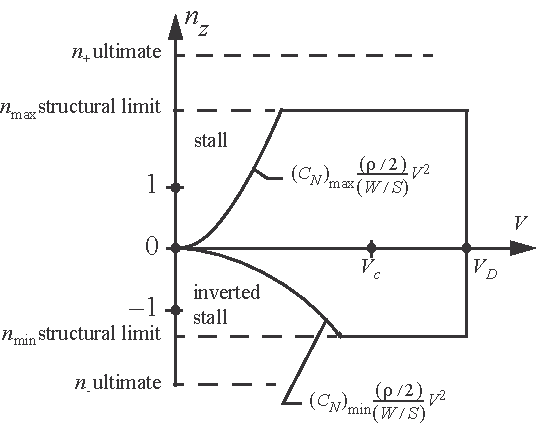
\includegraphics{Figure_2-14.pdf}
}{\caption{Maneuver V-n diagram including aerodynamic stall and\break specified data.\label{fig2.14}}}}



\noindent Note:\vspace*{-9pt}
\begin{enumerate}
\item[1.] $C_{N}$ varies with compressibility, and varies with the C.G. location as shown in eq. (\ref{eq2.41}). Generally we must consider different altitudes and weight configurations.

\item[2.] For flight in incompressible air, the dynamic pressure $q=\frac{1}{2} \rho V^{2}$, where $V$ is the airspeed and $\rho$ is the air density, both at altitude. Define \textbf{equivalent airspeed} $V_{\mathrm{EAS}}$ at sea level by
\begin{align}\label{eq2.46}
q=\frac{1}{2} \rho V^{2} \equiv \frac{1}{2} \rho_{\text {s.l. }} V_{\text {EAS }}^{2}.
\end{align}
Then the equivalent airspeed is given by $V_{\mathrm{EAS}}=\sqrt{\frac{\rho}{\rho_{\mathrm{s}.1}}} V$. Use $V_{\mathrm{EAS}}$ on V-n diagram to cover all altitudes. Some typical values of the load factors are shown in table 2.1\end{enumerate}

%Table 2.1		
\begin{table}[!h]
\processtable{Structural limit load factors\label{tab2.1}}
{\begin{tabular}{@{}lcc}\toprule
 & \multicolumn{2}{c}{\bf Structural limits}\\
 {\bf Category}	& {\bfseries\itshape n}$_{\textbf{max}}$ & {\bfseries\itshape n}$_{\textbf{min}}$\\\midrule
U.S. civil transports (Boeing) & 2.5 & $-1.0$\\
U.S. military heavy bomber	& 3.0 & $-1.0$\\
U.S. military subsonic attack	& 8.0 & $-3.0$\\
U.K. civil aerobatic & 6.0 & $-3.0$\\
U.K. sailplane, aerobatic & 7.0 & $-5.0$\\\botrule
\end{tabular}}{}
\vspace*{-16pt}
\end{table}

\paragraph{Transport category airplanes.}

The airworthiness standards for transport category airplanes are specified in Part 25 of the Federal Aviation Regulations (FAR). Flight maneuver and gust conditions are specified in subsections 25.331--25.351. The maneuver V-n diagram is shown in figure \ref{fig2.15}. The strength requirements must be met at each combination of airspeed and load factor on and within the boundaries of the representative maneuvering envelope (V-n diagram). The stalling speed with the flaps retracted at $n_{z}=1$ is denoted by $V_{s 1}$.

{\def\thefigure{2.15}
\processfigure[H]{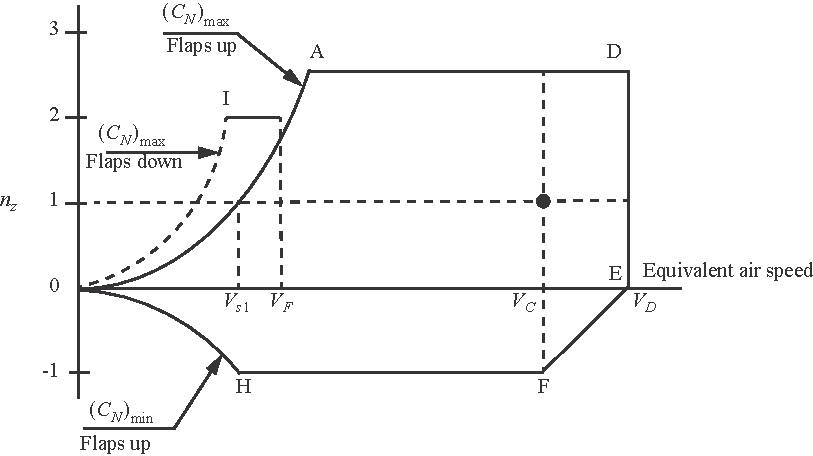
\includegraphics{Figure_2-15.pdf}
}{\caption{Flight maneuvering envelope per FAR 25.333.\label{fig2.15}}}}



\section{Design gust load factors}\label{sec2.5}

Turbulent conditions of varying intensity occur in air through which an airplane flies. For example, atmospheric phenomena that create turbulence are thermals (convection), mountain waves (terrain effects), wind shears, and jet streams. Assume steady level flight from still air, \textit{n = 1}, into an ideal sharp-edged gust as shown in figure \ref{fig2.16}\vadjust{\vfill\pagebreak}.

{\def\thefigure{2.16}
\processfigure[H]{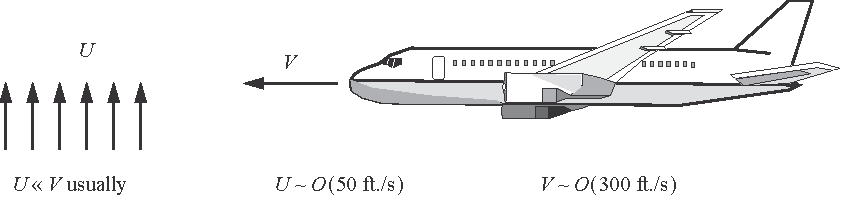
\includegraphics{Figure_2-16.pdf}
}{\caption{Steady level fight into a sharp-edged gust.\label{fig2.16}}}}


The change in the angle of attack due to the idealized sharp-edged gust is depicted in figure \ref{fig2.17}.

{\def\thefigure{2.17}
\processfigure{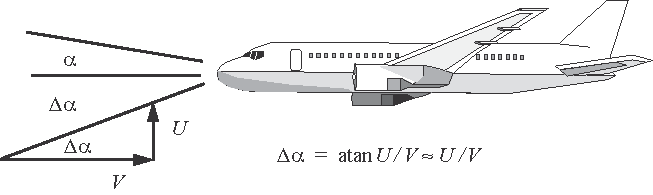
\includegraphics{Figure_2-17.pdf}
}{\caption[H]{Equivalent relative wind.\label{fig2.17}}}}


The lift curve slope between stall points is $m=\left(d C_{N}\right) /(d \alpha)$. Therefore, the change in the aerodynamic coefficient is
\begin{align}\label{eq2.47}
\Delta C_{N}=m(\Delta \alpha),
\end{align}
and the change in lift is
\begin{align}\label{eq2.48}
\Delta \mathrm{Lift}=\left(\frac{1}{2} \rho V^{2}\right) S m(\Delta \alpha)=\frac{1}{2} \rho V S\,m U.
\end{align}
Now the change in the load factor due to the gust is
\begin{align}\label{eq2.49}
\Delta n=\frac{\Delta \mathrm{Lift}}{W}=\left[\frac{(\rho m)/2}{(W/S)}\right] U V,
\end{align}
where $W/S$ is the wing loading in\,lb./ft.$^2$ The change in the load factor $\Delta n$ varies linearly with airspeed \textit{V} as depicted in figure \ref{fig2.18}.

%{\def\thefigure{2.18}
\begin{wrapfigure}[6]{r}{202pt}
\vspace{-30pt}
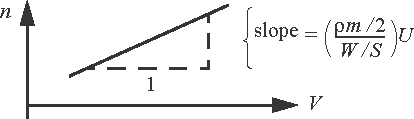
\includegraphics{Figure_2-18.pdf}
\caption{The linear change in the load factor.\label{fig2.18}}
\end{wrapfigure}
%}



\subsection{Gust alleviation factor}\label{sec2.5.1}

A more realistic, semiempirical treatment of gust effects, based on experience and analysis, is to replace the sharp-edge gust speed $U$ by $K_{g} U$, where $K_{g}$ is the gust alleviation factor. In reality there is no such thing as a sharp-edged gust so we account empirically for gust build-up and airplane response. For transport airplanes, NACA specified
\begin{align}\label{eq2.50}
K_{g}=\frac{0.88 \mu_{g}}{5.3+\mu_{g}}<0.88,
\end{align}
where $\mu_{g}$ is the airplane mass ratio defined by\vspace*{-9pt}
\begin{align}\label{eq2.51}
\mu_{g} \equiv \frac{W/S}{(\rho \bar{c} g m)/2},
\end{align}
and where $\bar{c}$ is the mean aerodynamic chord; $\bar{c}=S/b$, and $b$ is the wing span. See figure \ref{fig2.19}.

{\def\thefigure{2.19}
\begin{figure}
\centering{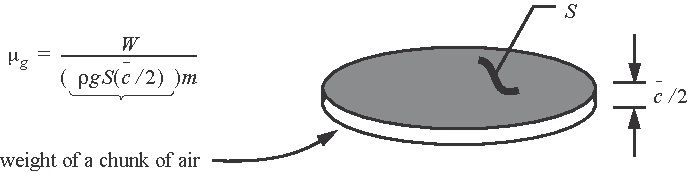
\includegraphics{Figure_2-19.pdf}}
\caption{Depiction of the airplane mass ratio.\label{fig2.19}}
\end{figure}}

%\vspace*{-12pt}


\subsection{Gust load factor}\label{sec2.5.2}

For steady level flight, the gust load factor is
\begin{align}\label{eq2.52}
\boxed{n=1+\left(\frac{\rho m/2}{W/S}\right) K_{g} U V.}
\end{align}
Note that a lightly loaded airplane is more susceptible than when heavily loaded. This is because the increment in lift is independent of the weight. A heavily loaded airplane has more inertia with which to smooth out gusts than a lightly loaded airplane, all other things being equal.

\subsection{NACA discrete gust conditions}\label{sec2.5.3}

Discrete gusts refer to sudden changes, or alleviated sharp-edged gusts, as opposed to continuous turbulence aircraft gust analysis. In continuous turbulence gusts are represented as a stationary Gaussian random process leading to specification of a power spectral density (Hoblit, 1988). For civil transport airplanes 0--20,000\,ft., three discrete gusts are specified:
\begin{enumerate}
\item[1.] Rough air gust: $U=66\,\mathrm{ft}/\mathrm{s}$ at $V=V_{B}$ a speed related to the stall speed.
\item[2.] High speed gust: $U=50\,\mathrm{ft}/\mathrm{s}$ at cruise speed $V_{C}$.
\item[3.] Dive speed gust: $U=25\,\mathrm{ft}/\mathrm{s}$ at dive speed $V_{D}$.
\end{enumerate}

The gust V-n diagram is shown in figure \ref{fig2.20}, and it is almost symmetrical with \textit{n = 1} line since gusts are as likely to act down as up.

{\def\thefigure{2.20}
\processfigure{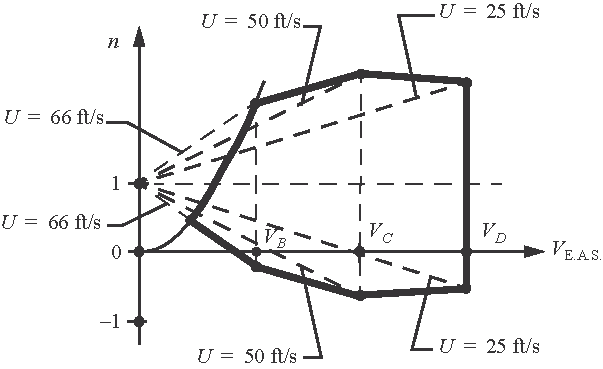
\includegraphics{Figure_2-20.pdf}
}{\caption{Gust V-n diagram.\label{fig2.20}}}}


\subsection{Design V-n diagram}\label{sec2.5.4}

The extreme load factors of both maneuver and gust diagrams must be met. Superimpose the two and take the outer boundaries as shown in figure \ref{fig2.21}. Generally, large airplanes are designed primarily by gust load factors. Small military and aerobatic airplanes are designed by maneuver load factors.

{\def\thefigure{2.21}
\processfigure{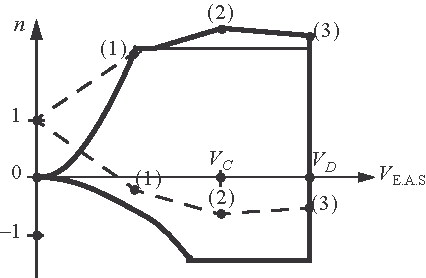
\includegraphics{Figure_2-21.pdf}
}{\caption{Design V-n diagram.\label{fig2.21}}}}


\section{Design V-n diagram example}\label{sec2.6}

This example is typical of a small aerobatic or perhaps military airplane, with specified data given figure \ref{fig2.22}.

{\def\thefigure{2.22}
\processfigure{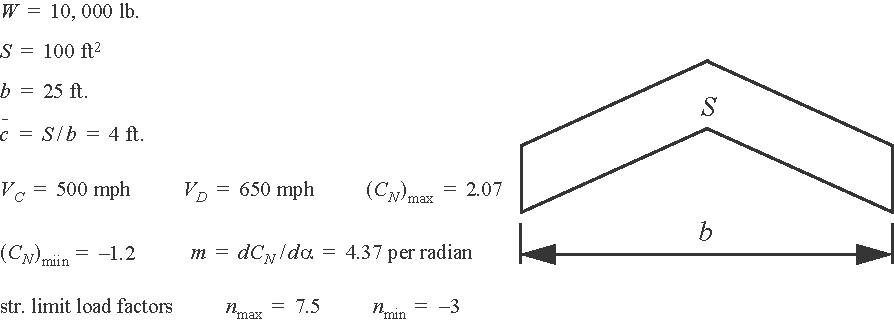
\includegraphics{Figure_2-22.pdf}
}{\caption{Data for the small aerobatic or military airplane.\label{fig2.22}}}}

\clearpage

\paragraph{Problem statement:}

Determine the design V-n diagram at sea level using the NACA formulas for gust loads.

\renewcommand\theequation{\alph{equation}}
\setcounter{equation}{0}

First, draw the maneuver V-n diagram. The stall boundary is given by
\begin{align}\label{ex2.6a}
n_{\text {stall }}=\left(C_{N}\right)_{\max } \frac{\rho_{\mathrm{s}.1.}/2}{W/S} V^{2}.
\end{align}
The density of air at sea level is
\begin{align}\label{ex2.6b}
\rho_{\text {s.l. }}=0.002378 \frac{\text { slugs }}{\mathrm{ft.}^{3}}\mbox{, where }1\,\mathrm{lb}.=(1 \mathrm{slug})(1\,\mathrm{ft}./\mathrm{s}^{2}).
\end{align}
The wing loading is
\begin{align}\label{ex2.6c}
W/S=(10,000 \text {lb.})/(100 \mathrm{ft.}^{2})=100\,\mathrm{lb}./\mathrm{ft}.^{2}.
\end{align}
Substitute eqs. (\textbf{\ref{ex2.6b}}) and (\textbf{\ref{ex2.6c}}) into eq. (\textbf{\ref{ex2.6a}}) to get
\begin{align}\label{ex2.6d}
n_{\text {stall }}=(2.07) \frac{\left(0.002378 \frac{\mathrm{lb} \cdot \mathrm{s}^{2}}{\mathrm{ft}.^{4}}/ 2\right)}{100\,\mathrm{lb}./\mathrm{ft}.^{2}} V^{2},\mbox{ or}\\
n_{\text {stall }}=2.46 \times 10^{-5}\,{V}^{2} \quad V~\text{in}\,\mathrm{ft}./\mathrm{s}.
\end{align}
The inverted stall boundary is
\begin{align}\label{ex2.6e}
n_{\text {istall }}=\left(C_{N}\right)_{\min } \frac{\rho_{\mathrm{s}.1.}/2}{W/S} V^{2}=\frac{-1.2(0.002378/2)}{100} V^{2},\mbox{ or}\\
n_{\text {istall }}=-1.43 \times 10^{-5} V^{2} \quad V~\text{in}\,\mathrm{ft}./\mathrm{s}.\label{ex2.6f}
\end{align}
The airspeeds at stall and structural limit factors are
\begin{align}\label{ex2.6g}
2.46 \times 10^{-5} V_{T}^{2}=7.5 \quad V_{T}=552\,\mathrm{ft}./\mathrm{s}\left(\frac{60\,\mathrm{mph}}{88\,\mathrm{ft}./ \mathrm{s}}\right)=376\,\mathrm{mph},\mbox{ and}\\
-1.43 \times 10^{-5}\left(V_{T}^{\prime}\right)^{2}=-3.0 \quad V_{T}^{\prime}=459\,\mathrm{ft}./ \mathrm{s}=313\,\mathrm{mph}.\label{ex2.6h}
\end{align}
The maneuver V-n diagram is shown in figure \ref{fig2.23}.

{\def\thefigure{2.23}
\def\floataboveskip{-3pt}
\processfigure{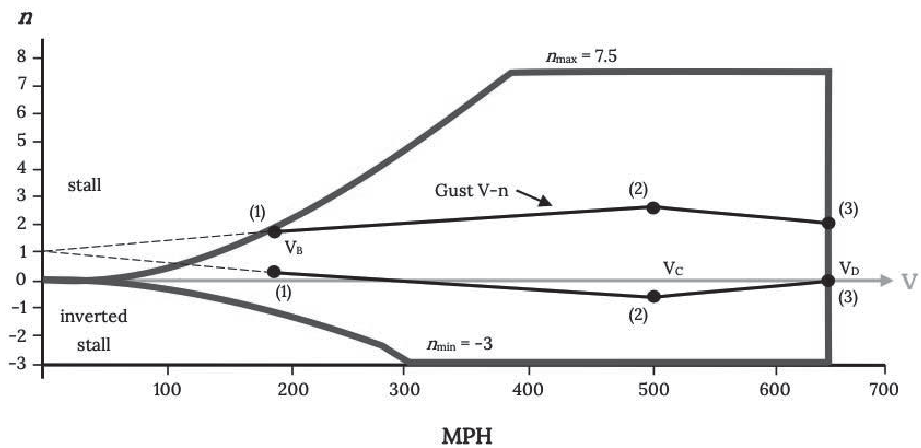
\includegraphics{Figure_2-23.pdf}
}{\caption{Maneuver and gust V-n diagrams for the example of a small aerobatic or military airplane.\label{fig2.23}}}}


Second, draw the gust V-n diagram using NACA formulas. Find the value of the gust alleviation factor as given in eq. (\ref{eq2.50}). The airplane mass ratio is
\begin{align}\label{ex2.6i}
\mu_{g} \equiv \frac{W/S}{(\rho \bar{c} g m)/2}&=\frac{100\,\mathrm{lb}./\mathrm{ft}^{2}}{(0.002378\,\mathrm{lb} \mathrm{s}^{2}/\mathrm{ft}^{4})(4\,\mathrm{ft}.)(32.2\,\mathrm{ft}/\mathrm{s}^{2})(4.37)/2},\mbox{ where}\\
\mu_{g}&=149\quad\mbox{dimensionless.}\nonumber
\end{align}
Hence, the gust alleviation factor is $K_{g}=0.85$. The change in the load factor due to the gust is
\begin{align}
\Delta n_{\text {gust }}&=\left(\frac{\rho m/2}{W/S}\right) K_{g} U V=\frac{0.002378(4.37)/2}{100}(0.85) U V,\mbox{ or}\label{ex2.6k}\\
\Delta n_{\text {gust }}&=4.42 \times 10^{-5} U V \quad U, V~\text{in}\,\mathrm{ft}./\mathrm{s}.\label{ex2.6l}
\end{align}
For gust (1) $U=66\,\mathrm{ft}/\mathrm{s}$ at $V=V_{B}$. To find the airplane speed $V_{B}$ on the stall boundary we set the load factor in eq. (2.52) equal to its relationship to the airplane speed on the stall boundary; i.e.,
\begin{align}\label{ex2.6m}
\underbrace{2.46 \times 10^{-5} V_{B}^{2}}_{\text {stall }}=1+\underbrace{4.42 \times 10^{-5}(66)}_{2.91 \times 10^{-3}} V_{B}.
\end{align}
Solve eq. (m) for speed $V_{B}$ as follows:
\begin{align}\label{ex2.6n}
V_{B} &=\frac{2.91 \times 10^{-3} \pm \sqrt{\left(2.91 \times 10^{-3}\right)^{2}+4\left(2.46 \times 10^{-5}\right)(1)}}{2\left(2.46 \times 10^{-5}\right)},\nonumber\\
V_{B}&=\frac{2.91 \times 10^{-3} \pm 1.03 \times 10^{-2}}{2\left(2.46 \times 10^{-5}\right)}\quad\mbox{choose} +.
\end{align}
Hence, $V_{B}=269\,\mathrm{ft}/\mathrm{s}=184\,\mathrm{mph}$, and the change in load factor for gust (1) is
\begin{align}\label{ex2.6o}
\Delta n_{1}=4.42 \times 10^{-5}(66)(269)=0.78.
\end{align}
For gust (2) $U=50\,\mathrm{ft}/\mathrm{s}$ at $V_{C}=500\,\mathrm{mph}$. Hence, the change in load factor is
\begin{align}\label{ex2.6p}
\Delta n_{2}=4.42 \times 10^{-5}(50)\left[500\,\mathrm{mph}\left(\frac{88\,\mathrm{ft}/ \mathrm{s}}{60\,\mathrm{mph}}\right)\right]=1.62.
\end{align}
For gust (3) $U=25\,\mathrm{ft}/\mathrm{s}$ at 650\,mph, and the change in load factor is\pagebreak
\begin{align}\label{ex2.6q}
\Delta n_{3}=4.42 \times 10^{-5}(25)\left[650\,\mathrm{mph}\left(\frac{88\,\mathrm{ft}/ \mathrm{s}}{60\,\mathrm{mph}}\right)\right]=1.05.
\end{align}
Thus, the six points on the gust V-n diagram are
\begin{align}\label{ex2.6r}
\begin{array}{ll}
1 \pm \Delta n_{1}=1.78,0.22 & V_{B}=184\,\mathrm{mph} \\
1 \pm \Delta n_{2}=2.62,-0.62 & V_{C}=500\,\mathrm{mph} \\
1 \pm \Delta n_{3}=2.05,-0.05 & V_{D}=650\,\mathrm{mph}
\end{array}.
\end{align}
A sketch of the gust V-n diagram is shown in figure \ref{fig2.23}. Here the design V-n diagram is the maneuver V-n diagram since the gust V-n diagram is contained inside the maneuver V-n diagram.


\begin{thebibliography}{}
\bibitem{}
Hoblit, F.M., \textbf{\textit{Gust Loads on Aircraft: Concepts and Applications}}. Reston, VA: American Institute of Aeronautics and Astronautics, Inc., 1988.

\bibitem{}\label{Lomax}
Lomax, T. L., \textbf{\textit{Structural Loads Analysis for Commercial Transport Aircraft: Theory and Practice}}. Reston, VA: American Institute of Aeronautics and Astronautics, Inc., 1996.

\bibitem{}\label{Megson}
Megson, T.H.G., \textbf{\textit{Aircraft Structures for Engineering Students}}, 3d ed., New York: John Wiley \& Sons Inc.; London: Arnold, a member of the Hodder Headline Group, 1999.

\bibitem{}\label{Peery}
Peery, D. J., 2011, \textbf{\textit{Aircraft Structures}}. Dover Publications, Inc., 2011. (Unabridged republication of the work originally published in 1950 by the McGraw-Hill Book Company, New York.) Chapter 3.
\end{thebibliography}

\section{Practice exercises}\label{sec2.7}

\begin{enumerate}
\item[1.] An airplane weighting 8,000\,lb. has an upward acceleration of 3g when landing. If the dimensions are as shown in figure 2.24, what are the wheel reactions $R_{1}$ and $R_{2}$? What is the time required to decelerate the airplane from a vertical velocity of 12\,ft./s? What is the shear and bending moment on a vertical section A--A, if the weight forward of this section is 2,000\,lb. and has a center of gravity 40\,in. from this cross section. (Peery, 2011,~p.~54).

{\def\thefigure{2.24}
\processfigure{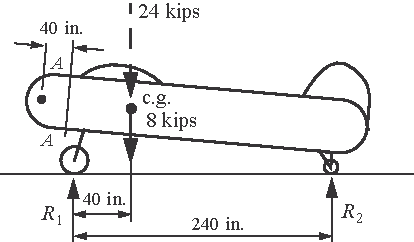
\includegraphics{Figure_2-24.pdf}
}{\caption{Exercise 1.\label{fig2.24}}}}


\item[2.] An 8,000\,lb. airplane is making a horizontal turn with a radius of 1,000\,ft. and with no change in altitude. See figure \ref{fig2.25}. Find the angle of bank and the load factor for a speed of (a) 200\,mph., (b) 300\,mph, and (c) 400\,mph. Find the loads on the wing and tail if the dimensions are as shown (Peery, 2011, p. 72).

\pagebreak

{\def\thefigure{2.25}
\begin{figure}
\centering{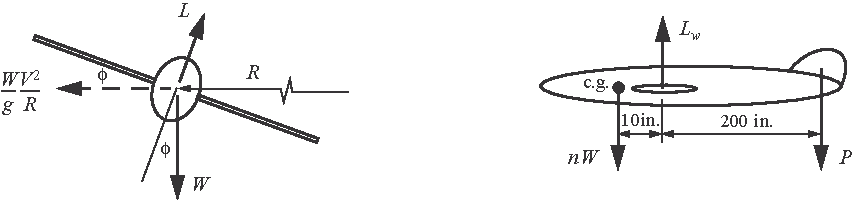
\includegraphics{Figure_2-25.pdf}}
\caption{Exercise 2. Level flight coordinated turn.\label{fig2.25}}
\end{figure}
}



\vspace*{-12pt}

\item[3.] The airplane shown in figure \ref{fig2.26} is making an arrested landing on a carrier deck. At the position shown, the angular velocity is 0.5 rad/s counterclockwise and the vertical velocity of the center of gravity is 12\,ft./s. The radius of gyration for the mass of the airplane about the center of gravity is 60\,in. Find the load factors $n_{x}$ and $n_{y}$, parallel and perpendicular to the deck, for a point at the center of gravity, a point 200\,in. aft of the center of gravity, and a point 100\,in. forward of the center of gravity. Find the vertical velocity with which the nose wheel strikes the deck. Assume no change in the dimensions or loads, and the downward acceleration of the nose wheel is constant in the 10\,in. of vertical travel (Peery, 2011, p. 72).


{\def\thefigure{2.26}
\processfigure{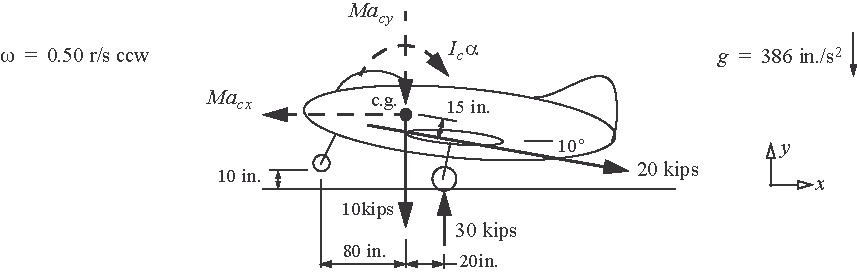
\includegraphics{Figure_2-26.pdf}
}{\caption{Exercise 3. Arrested landing on a carrier deck.\label{fig2.26}}}}

\vspace*{-10pt}

\item[4.] The aircraft shown below weighs 135\,kN and has landed such that at the instant of impact the ground reaction on each main undercarriage wheel is 200\,kN and its vertical velocity is 3.5\,m/s.  (Adapted from Megson, 1999, P.8.1, p. 272.)

{\def\thefigure{2.27}
\processfigure{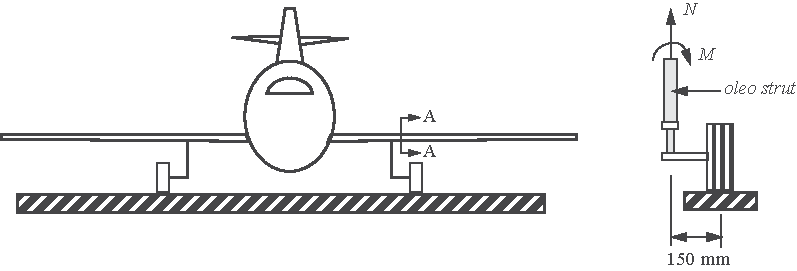
\includegraphics{Figure_2-27.pdf}
}{\caption{Exercise 4: Instant of impact upon landing.\label{fig2.27}}}}

\medskip

Each undercarriage wheel weighs 2.25\,kN and is attached to an oleo strut.

\medskip

\begin{enumerate}[d)]
\item[a)] What is an oleo strut? What is its purpose? Describe is components and how it functions.

\item[b)] Calculate the axial load \textit{N} and bending moment \textit{M} in the strut, assuming the strut is vertical.

\item[c)] Determine the shortening of the strut when the vertical velocity of the aircraft is zero.

\item[d)] Calculate the shear force and bending moment in the wing section A-A if the wing outboard of section A-A weighs 6.6\,kN and has a center of gravity 3.05\,m from A-A.
\end{enumerate}

\item[5.] An airplane has a \textbf{total} weight of 40,000\,lb. and \textbf{total} \textbf{rolling} moment of inertia about the C.G. of 1,000,000\,lb.-s$^2$-in. Each wing-tip store weighs 2,000\,lb. In steady level flight, each wing's resultant lift is $L_{w}=21{,}000$\,lb. (The tail carries stabilizing a negative lift of 2,000\,lb.) In a sudden evasive roll maneuver from steady level flight, each aileron introduces a lift increment $L_{a}=\pm 3,000$\,lb. Assuming the airplane to be rigid and, neglecting wing weight, calculate the total root bending moment for each wing (i.e., $M_{A}$ and $M_{B}$). Neglect the moment of inertia of each wing-tip store about its own C.G.

    {\def\thefigure{2.28}
\processfigure[H]{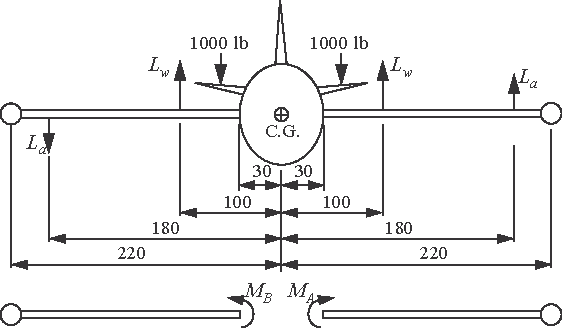
\includegraphics{Figure_2-28.pdf}
}{\caption{Exercise 5: Evasive roll maneuver from steady level flight.\label{fig2.28}}}}


\item[6.] Use the data given in table \ref{tab2.2} and the NACA gust formulas to develop the design V-n diagram for the Boeing 727 aircraft at sea level. The airspeed should be in\,knots. One\,knot equals one nautical mile per hour, and approximate one nautical mile as 6,080~ft.\footnote{A nautical mile is based on the circumference of the planet Earth. If you were to cut the Earth in half at the equator, you could pick up one of the halves and look at the equator as a circle. You could divide that circle into 360 degrees. You could then divide a degree into 60 minutes. A minute of arc on the planet Earth is 1 nautical mile. This unit of measurement is used by all nations for air and sea travel. A nautical mile is 1,852 meters, or 1.852 kilometers. In the English measurement system, a nautical mile is 1.1508 miles, or 6,076 feet. [http://www.howstuffworks.com]}  Clearly label the plot. Also calculate the level flight stall speed $V_{S 1}$.


%Table 2.2		
\begin{table}[!h]
\processtable{Exercise 6\label{tab2.2}}
{\begin{tabular}{@{}ll}\toprule
$S$	& 1560\,ft.$^{.2}$\\
$b$	& 108\,ft.\\
$W$	& 170,000\,lb.\\
$(d C_{z a})/(d \alpha)$	& 5.0 per radian\\
$C_{z a \max}$ & 0.951\\
$C_{z a \min}$ & $-0.400$\\
$n_{\max}$	& 2.5 (structural)\\
$n_{\min}$	& $-1.0$ (structural)\\
$V_{\rm C}$ & 350\,kNots\\
$V_{\rm D}$ & 440\,kNots\\\botrule
\end{tabular}}{\vspace*{-60pt}}
\end{table}

\item[7.] Shown below is the maneuver V-n diagram at sea level for an aircraft of wing span 27.5\,m, mean aerodynamic chord 3.05 m, and total weight 196,000\,N. The aerodynamic center is 0.915\,m forward of the center of gravity and the center of lift for the tail unit is 16.7\,m aft of the C.G. The pitching moment coefficient is
\begin{align*}
C_{\mathrm{M} 0.25}=-0.0638(\text{nose-up positive}).
\end{align*}
Both the pitching moment coefficient and the position of the aerodynamic center are specified for the complete aircraft less the tail unit\vadjust{\vspace*{15pt}\pagebreak}.

{\def\thefigure{2.29}
\processfigure[H]{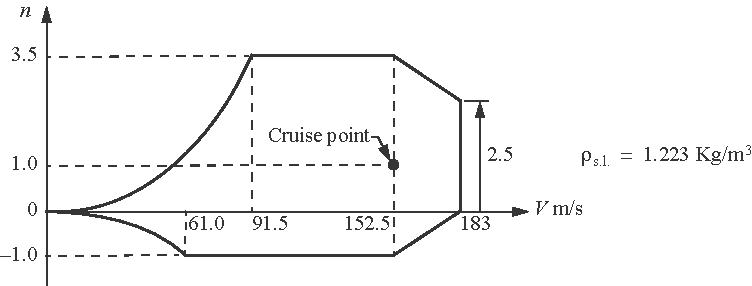
\includegraphics{Figure_2-29.pdf}
}{\caption{Exercise 7: Maneuver V-n diagram at sea level (U.K. regulations).\label{fig2.29}}}}

For steady level flight at sea level the fuselage bending moment at the C.G. was recorded by test equipment to be 600,000\,N m. Calculate the maximum value of this bending moment for the given flight envelope, or V-n diagram. For this purpose it may be assumed that the aerodynamic loadings on the fuselage structure itself can be neglected; i.e., the only loads on the fuselage aft of the C.G. are those due to tail lift and the inertia of the fuselage.
\end{enumerate}

\clearemptydoublepage

\end{document}